% Copyright (C)  2013 Jana Traue (jana.traue[at]tu-cottbus.de)
%
% Permission is granted to copy, distribute and/or modify this document
% under the terms of the GNU Free Documentation License, Version 1.3
% or any later version published by the Free Software Foundation;
% with no Invariant Sections, no Front-Cover Texts, and no Back-Cover Texts.
% A copy of the license is included in the file entitled "LICENSE".
%
% =============================================================================
\section{Examples}
% =============================================================================
%
% -----------------------------------------------------------------------------
\subsection{Code Listings}
% -----------------------------------------------------------------------------
\label{demo:examples:listings}
%
This (\ref{lst:CodeExample}) is an example for listings.
%
\begin{lstlisting}[label={lst:CodeExample},     
 caption={Code Example (\code{HelloWorld.cpp})}]
void test()
{
    cout << "Hello World" << endl;
}
\end{lstlisting}
%
%
It is possible to specify the start of line numbers.
%
\begin{lstlisting}[label={lst:CodeExample2},     
 caption={Changed Numbering (\code{HelloWorld.cpp})},
 firstnumber=20]
void test()
{
    cout << "Hello World" << endl;
}
\end{lstlisting}
%
This document defines C++ as the default code language
and highlights keywords.
The correspondig settings can be found in \code{header.tex}.
Take a look at the 
\href{http://www.ctan.org/tex-archive/macros/latex/contrib/listings/}
{CTAN documentation} for further information
about listings.
%
% -----------------------------------------------------------------------------
\subsection{Figures}
% -----------------------------------------------------------------------------
%
% .............................................................................
\subsubsection{Placement}
% .............................................................................
If no placement option is specified, figures show up at unexpected places.
Use a combination of the following options:
\begin{itemize}
    \item h: where the figure is created in the source code
    \item t: top of a page
    \item b: bottom of a page
    \item p: on a separate page
\end{itemize}
%
% .............................................................................
\subsubsection{Simple Figures}
% .............................................................................
%
Figure \ref{fig:SimpleFigure} shows a simple figure.
%
\begin{figure}[htb]
	\begin{center}
		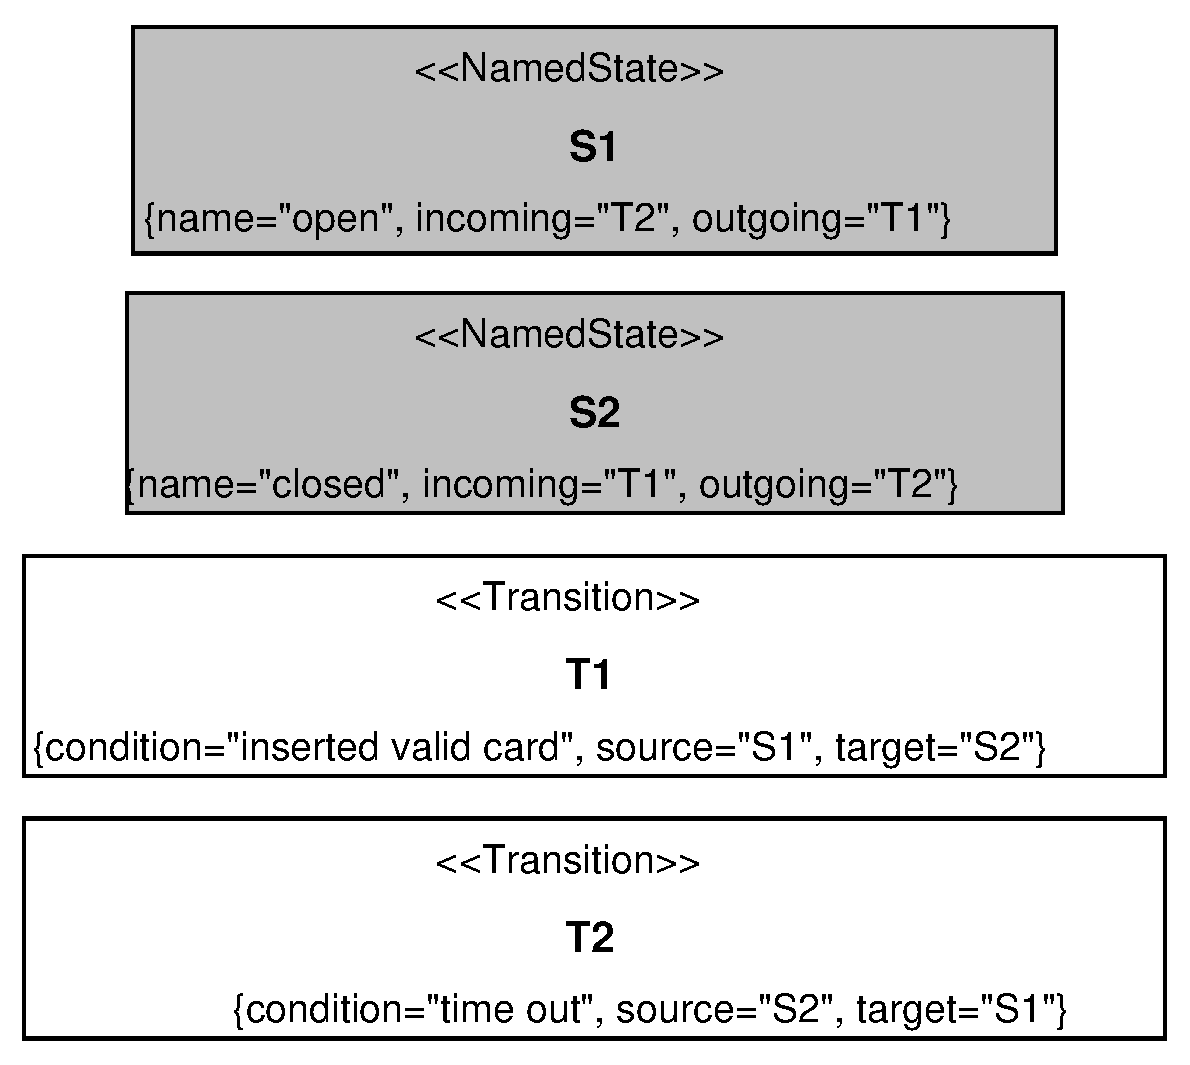
\includegraphics[scale=0.4]{demo/Version2-M1-2}
		\caption{Simple Figure}
		\label{fig:SimpleFigure}
	\end{center}
\end{figure}
%
%
% .............................................................................
\subsubsection{Multiple Figures}
% .............................................................................
%
Figures \ref{fig:MultiFigureA} and \ref{fig:MultiFigureB} show how two place 
two figures side by side.
%
\begin{figure}[htb]
	\begin{center}
		\subfigure[left figure] {
			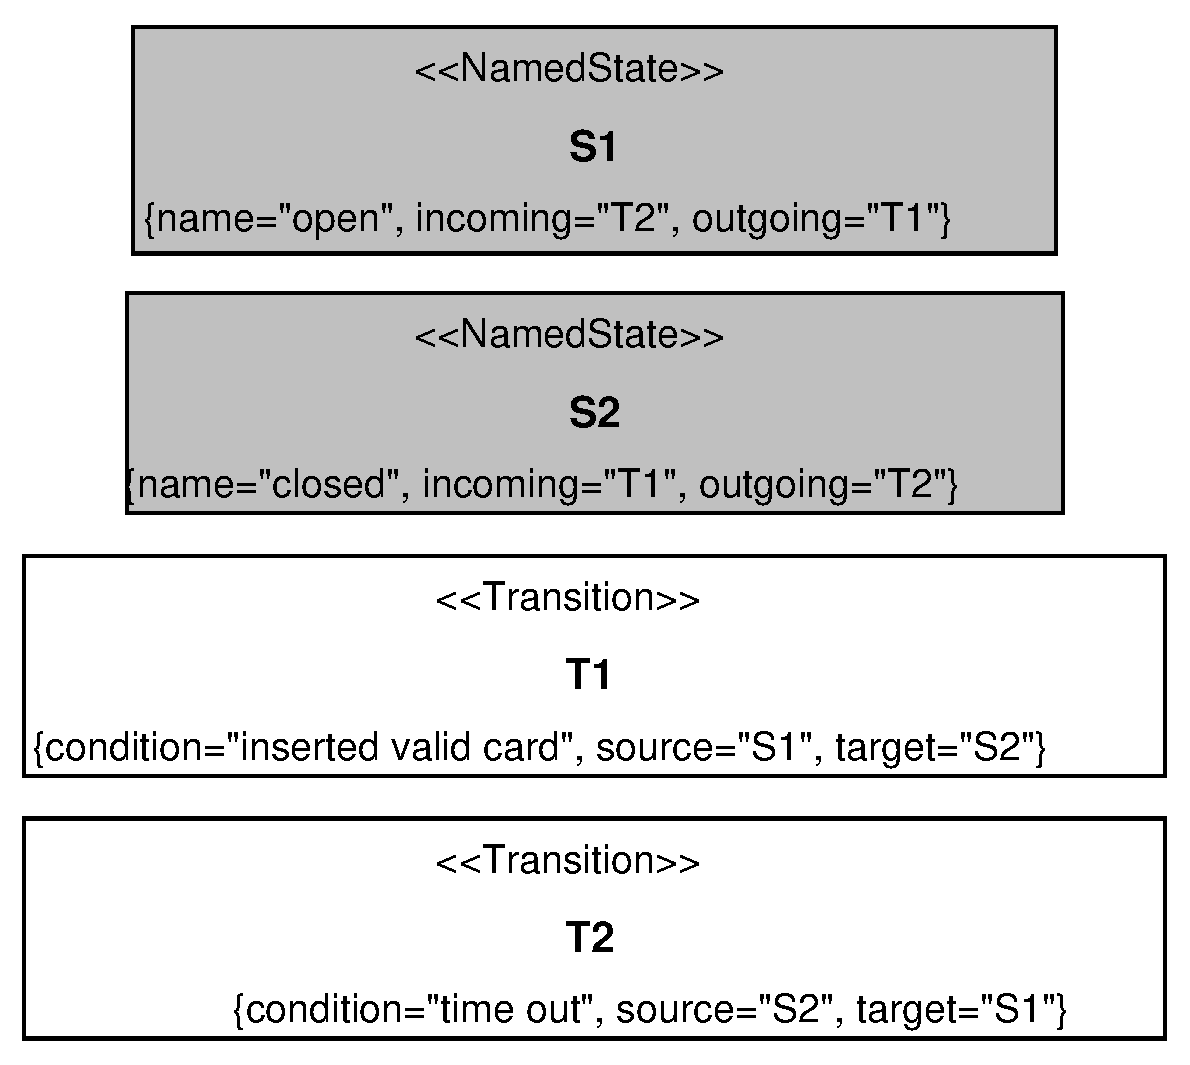
\includegraphics[scale=0.4]{demo/Version2-M1-2}	
			\label{fig:MultiFigureA}
		}
		\subfigure[right figure] {
			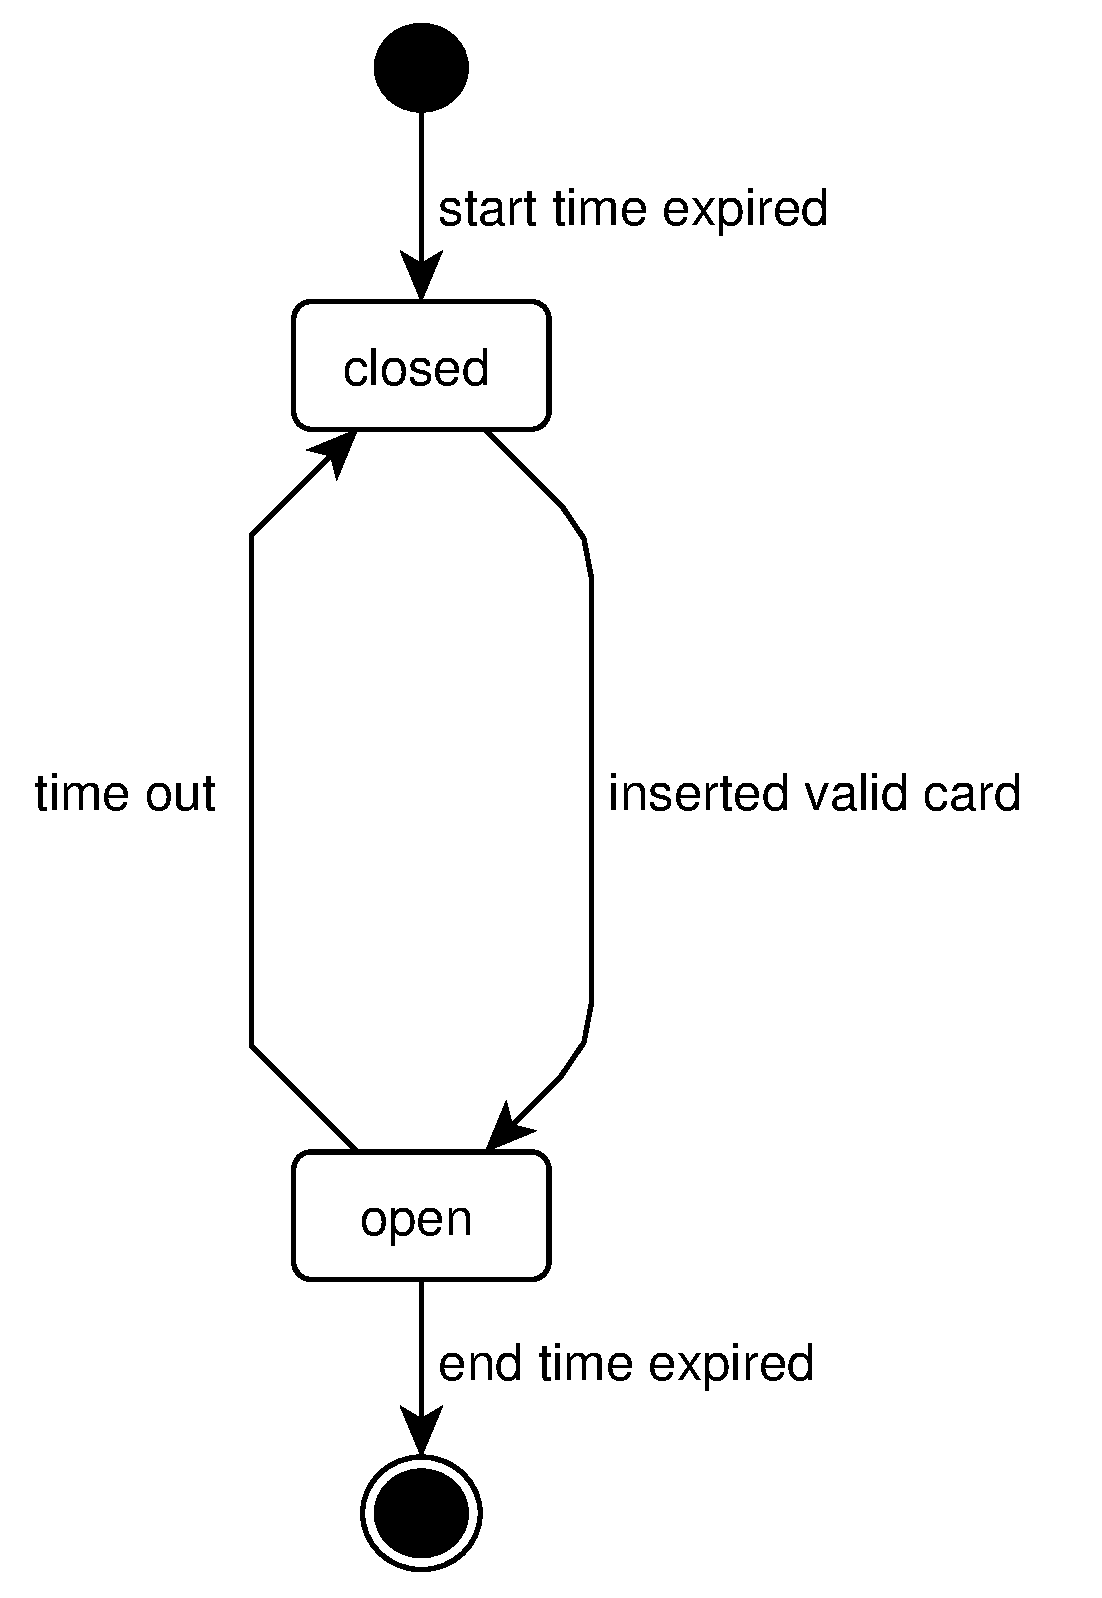
\includegraphics[scale=0.3]{demo/Version2-M1-1}
			\label{fig:MultiFigureB}
		}
		\caption{Two Figures Side by Side}
	\end{center}
\end{figure}
%
% -----------------------------------------------------------------------------
\subsection{TODO Notes}
% -----------------------------------------------------------------------------
%
It is possible to add todo\todo{Example} notes to a text.
This might be useful on reviewing documents or mark sections
which should be rewritten.
Sometimes it is useful to place them in-line like this:
\todo[inline]{An in-line todo note.}
%
It is possible to list all todo items.
\listoftodos
%
% -----------------------------------------------------------------------------
\subsection{Citations}
% -----------------------------------------------------------------------------
%
The \code{bib} folder contains an example bibliography file.
It includes bib entries for a book\cite{LatexBook} and
a website\cite{LatexWebsite}
%
% -----------------------------------------------------------------------------
\subsection{Tikz Graphics}
% -----------------------------------------------------------------------------
%
This section shows some examples for graphics which are not included
from external files. Instead, the \href{http://www.texample.net/tikz/}
{tikz} package is used.
Seems not very handy - still looking for better solutions.
% .............................................................................
\subsubsection{Stack Frame using tikz}
% .............................................................................
%
\newcommand{\frameheight}{0.6cm}
\newcommand{\framewidth}{3cm}
\begin{tikzpicture}[%
	start chain=1 going below,
	node distance=0cm,
	outer sep = 0pt]
	\tikzstyle{content}=[	% style for stack content
		draw, 				%
		rectangle,  		%
		minimum height=\frameheight,% 
		minimum width=\framewidth,% 
		fill=blue!20,		%
		anchor=north east	%
	]
	\tikzstyle{address}=[	%
		draw=none, 			%
		rectangle, 			%
		minimum height=\frameheight,% 
		minimum width=\framewidth,% 		
		fill=yellow!30,		%
		anchor=north east]	%
	\tikzstyle{space}=[	%
		draw=none, 			%
		rectangle, 			%
		minimum height=\frameheight,% 
		minimum width=\framewidth,% 		
		fill=red!30,		%
		anchor=north east]	%
\tikzstyle{arrow}=[	%
		draw=none, 			%
		rectangle, 			%
		minimum height=\frameheight,% 
		minimum width=0.7\framewidth,% 		
		fill=red!30,		%
		anchor=north east]	%		
%	
\node[address, on chain=1] 	(a0128)						{0x0128};
\node[content] 				(c0128) [right = of a0128]	{R0};	
%
\node[address, on chain=1] 	(a0127)						{0x0127};
\node[content] 				(c0127) [right = of a0127]	{R1};	
%
\node[space, on chain=1] 	(aSEP1) 					{};
\node[space]				(cSEP1) [right = of aSEP1]  {};
\draw (cSEP1.north west) -- (cSEP1.west);
\draw[snake=coil,segment aspect=0, segment length=30] (cSEP1.west) -- (cSEP1.east); 
\draw (cSEP1.north east) -- (cSEP1.east);
%
\node[space, on chain=1] 	(aSEP2) 					{};
\node[space]				(cSEP2) [right = of aSEP2]  {};
%
\node[address, on chain=1] 	(a0098)						{0x0098};
\node[content] 				(c0098) [right = of a0098]	{R30};
%
\draw (cSEP2.south west) -- (cSEP2.west);
\draw[snake=coil,segment aspect=0, segment length=30] (cSEP2.west) -- (cSEP2.east); 
\draw (cSEP2.south east) -- (cSEP2.east);
%
\node[address, on chain=1] 	(a0097)						{0x0097};
\node[content] 				(c0097) [right = of a0097]	{R31};	
\node[address, on chain=1] 	(a0096)						{0x0096};
\node[content] 				(c0096) [right = of a0096]	{SREG};	
%
\node[address, on chain=1] 	(a0095)						{0x0095};
\node[content] 				(c0095) [right = of a0095]	{};	
%
% stack pointer
\node[arrow]				(SP)	[right = of c0095]	{};
\draw[<-, line width=2] (SP.west) -- (SP.east);
\node[arrow]				(SPL) 	[right = of SP]		{SP};

\end{tikzpicture}
%
% .............................................................................
\subsubsection{Stack Frame using tabular and tikz}
% .............................................................................
%
% define new style for data cells
% used to have borders around single cells and not whole lines or columns
\def\dataCell#1{ \multicolumn{1}{|c|}{#1}}
%
% table layout:
% address			& data			&	(used for placing nodes - for braces)
% (aligned right)	& (centered)	&	(aligned left)
\begin{tabular}{rcl} % alignment is: right, center, left
%
% header:
\textbf{adress}	& \textbf{data} &													\\
% contents:
% \cline{2-2} means that a horizontal line from column 2 to 2 is drawn
% stack pointer is currently defined in third column with: $\longleftarrow$ SP
% remember to use unique names for nodes and to adjust tikz picture below on changes
0x0129  & \dataCell{}		& 														\\\cline{2-2}
0x0128	& \dataCell{R0} 	& \tikz[remember picture] \node (startCoroutine1) {};	\\\cline{2-2}
0x0127	& \dataCell{R1} 	&														\\\cline{2-2}
0x0126	& \dataCell{R2} 	& 														\\\cline{2-2}
		& \ldots			&														\\\cline{2-2}
0x0098	& \dataCell{R30} 	&														\\\cline{2-2}
0x0097	& \dataCell{R31} 	&														\\\cline{2-2}
0x0096	& \dataCell{SREG} 	& \tikz[remember picture] \node (endCoroutine1) {};		\\\cline{2-2}
0x0195  & \dataCell{}		& $\longleftarrow$ SP									\\\cline{2-2}
\end{tabular} 
%
% paint braces
\begin{tikzpicture}[remember picture,overlay]
	% add a new node for the brace
	\node (braceCoroutine1) [right delimiter=\},fit=(startCoroutine1) (endCoroutine1)] {};
	% add a new node for the label
	\node [right of=braceCoroutine1,anchor=west] {context of coroutine 1};
\end{tikzpicture}  
%
% .............................................................................
\subsubsection{Graph using tikz}
See Figure \ref{fig:exampleGraph}
% .............................................................................
\tikzset
{
    NodeStyle/.style =
    {
        shape = ellipse,      % shape
        scale = 1.0,            % scaling factor
        % thick,                % thickness of the border
        %
	    % -- color properties --
        % filling: [ trasparent | monocolored | shaded]; decomment what you prefer
        %										% transparent (all commented)
        fill			= black!10!white,	    % monocolored
        % top color		= white,				% | filling of the node
        % bottom color	= red!50!black!20,		% |
        % text			= black,				% colour of the fonts
        draw			= black,				% colour of the border
		%
		% -- fonts --
        % font			= \scriptsize,  % shape of the font (or dimension, like \tiny)
        % text flushlefted,				% text alignment [text flushlefted | text badly flushlefted | text justified | text ragged | text badly ragged]
        % text height		= 1mm,		% ! minimum size of the text	% NOT WORKING
        % text depth		= 1mm,		% !
		% inner xsep		= 3mm,		% minimum distance between text and borders along x dimension
		% inner ysep		= 3mm		% minimum distance between text and borders along y dimension
    }
}
\begin{figure}[htb]
\begin{center}
\begin{tikzpicture}
[
    xscale = 1, % to scale horizontally everything but the text
    xscale = 1  % to scale vertically everything but the text
]
%
\node   (nodeA) [NodeStyle] {A};
\node   (nodeB) [NodeStyle, right = 2 of nodeA] {B};
\node   (nodeD) [NodeStyle, below = 2 of nodeA] {D};
\node   (nodeC) [NodeStyle, right = 2 of nodeD] {C};
\node   (nodeE) [NodeStyle, right = 2 of nodeC] {E};

\draw   (nodeA) to node [sloped, above] {5} (nodeB);
\draw   (nodeA) to node [sloped, above] {1} (nodeD);
\draw   (nodeB) to node [sloped, above] {2} (nodeC);
\draw   (nodeB) to node [sloped, above] {4} (nodeE);
\draw   (nodeD) to node [sloped, above] {2} (nodeC);
\draw   (nodeC) to node [sloped, above] {1} (nodeE);

\end{tikzpicture}
\caption{Demo Graph}
\label{fig:exampleGraph}
\end{center}
\end{figure}
%
% -----------------------------------------------------------------------------
\subsection{Bytefields}
% -----------------------------------------------------------------------------
%
The 
\href{http://www.ctan.org/tex-archive/macros/latex/contrib/bytefield/}
{bytefield package} is sometimes very handy.
This example is not included by default, because the bytefield package is
not part of the standard distributions and the file would
not compile without it.
Once you installed the package, uncomment the upcoming text.
%
% Figure \ref{fig:vmAddr} shows an example. The fields might be linked
% to textual items like that:
% % %
% \begin{description}
    % \item[\hypertarget{vmAddr:unused}{Unused}]:
        % Not used, because 32 bit paging is simulated.
    % \item[\hypertarget{vmAddr:pdIndex}{Page Directory Index}]:
        % Offset to an entry in the page directory.
        % The selected entry provides the base physical address of a
        % page table.
    % \item[\hypertarget{vmAddr:ptIndex}{Page Table Index}]:
        % Offset to an entry in the selected page table. This entry provides
        % the base physical address of a page in physical memory.
    % \item[\hypertarget{vmAddr:offset}{Offset}]:
        % Not used.
        % Offset to a physical address in the page.
% \end{description}
% %
%\begin{figure}[htb]
%  \begin{center}
%      \begin{bytefield}[bitwidth=0.6em, bitheight=6ex]{64}
%        \bitheader[b]{0,11-12,21-22,31-32,63} \\
%        \bitbox{32}{\hyperlink{vmAddr:unused}{Unused}} &
%            \bitbox{10}{\hyperlink{vmAddr:pdIndex}{PD index}} &
%            \bitbox{10}{\hyperlink{vmAddr:ptIndex}{PT index}} &
%            \bitbox{12}{\hyperlink{vmAddr:offset}{Offset}}
%      \end{bytefield}
%  \end{center}
%  \caption{Structure of a virtual 64 bit address}
%  \label{fig:vmAddr}
%\end{figure}
